\documentclass[tikz, border=0pt]{standalone}
\usepackage{libertinus}
\usepackage[T1]{fontenc}
\usepackage{microtype}
\usepackage{xcolor}

\definecolor{accent}{RGB}{20,90,80}
\definecolor{accentlight}{RGB}{230,240,238}
\definecolor{bookgray}{RGB}{96,102,111}
\definecolor{bg}{RGB}{247,247,244}

\begin{document}
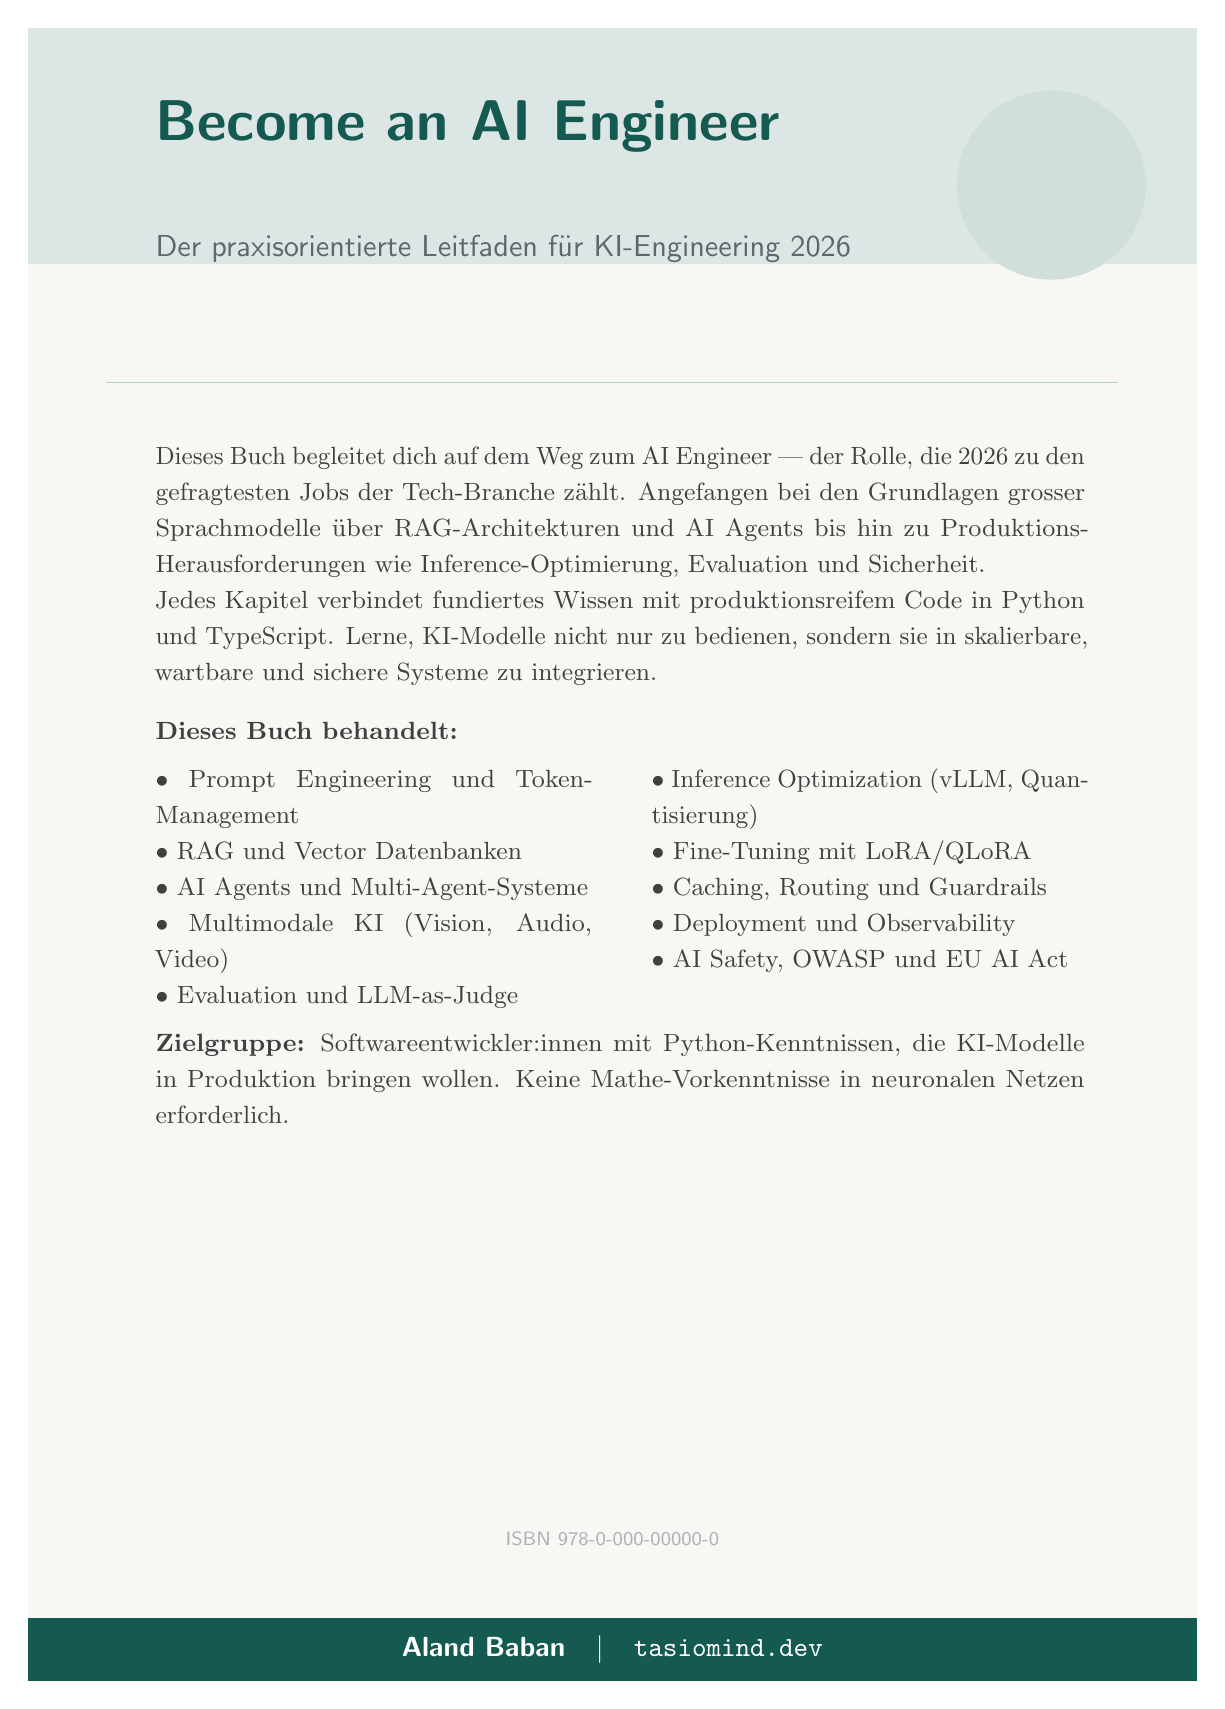
\begin{tikzpicture}
  \fill[bg] (0,0) rectangle (148.5mm,210mm);
  \fill[accent!15] (0,180mm) rectangle (148.5mm,210mm);
  \fill[accent] (0,0) rectangle (148.5mm,8mm);
  \draw[accent!30, line width=0.3pt] (10mm,165mm) -- (138.5mm,165mm);

  \node[align=left, text=accent, font=\fontsize{22}{26}\sffamily\bfseries] at (15mm,193mm) [anchor=south west] {Become an AI Engineer};
  \node[align=left, text=bookgray, font=\fontsize{11}{14}\sffamily] at (15mm,179mm) [anchor=south west] {Der praxisorientierte Leitfaden f\"ur KI-Engineering 2026};

  \node[align=left, text=black!75, font=\fontsize{9}{13}\rmfamily] at (15mm,158mm) [anchor=north west] {
    \parbox{118mm}{
    Dieses Buch begleitet dich auf dem Weg zum AI Engineer --- der Rolle, die
    2026 zu den gefragtesten Jobs der Tech-Branche z\"ahlt. Angefangen bei den
    Grundlagen grosser Sprachmodelle \"uber RAG-Architekturen und AI Agents bis
    hin zu Produktions-Herausforderungen wie Inference-Optimierung,
    Evaluation und Sicherheit.

    Jedes Kapitel verbindet fundiertes Wissen mit produktionsreifem Code in
    Python und TypeScript. Lerne, KI-Modelle nicht nur zu bedienen, sondern
    sie in skalierbare, wartbare und sichere Systeme zu integrieren.

    \vspace{3mm}
    \textbf{Dieses Buch behandelt:}

    \vspace{1.5mm}
    \begin{minipage}[t]{55mm}
    $\bullet$~Prompt Engineering und Token-Management\\
    $\bullet$~RAG und Vector Datenbanken\\
    $\bullet$~AI Agents und Multi-Agent-Systeme\\
    $\bullet$~Multimodale KI (Vision, Audio, Video)\\
    $\bullet$~Evaluation und LLM-as-Judge
    \end{minipage}
    \hfill
    \begin{minipage}[t]{55mm}
    $\bullet$~Inference Optimization (vLLM, Quantisierung)\\
    $\bullet$~Fine-Tuning mit LoRA/QLoRA\\
    $\bullet$~Caching, Routing und Guardrails\\
    $\bullet$~Deployment und Observability\\
    $\bullet$~AI Safety, OWASP und EU AI Act
    \end{minipage}

    \vspace{3mm}
    \textbf{Zielgruppe:} Softwareentwickler:innen mit Python-Kenntnissen,
    die KI-Modelle in Produktion bringen wollen. Keine Mathe-Vorkenntnisse
    in neuronalen Netzen erforderlich.
    }};

  \node[align=center, text=white, font=\fontsize{10}{12}\sffamily\bfseries] at (74.25mm,4mm) [anchor=center] {Aland Baban ~~$|$~~ \ttfamily tasiomind.dev};
  \node[align=center, text=bookgray!50, font=\fontsize{7}{9}\sffamily] at (74.25mm,16mm) [anchor=south] {ISBN 978-0-000-00000-0};
  \fill[accent!20] (130mm,190mm) circle (12mm);

\end{tikzpicture}
\end{document}
